\chapter{Estado del arte.}\label{sec:estadodelarte}

\paragraph{}En este capítulo se va a tratar el estado actual de las tecnologías
más relevantes para llevar a cabo entornos de desarrollo replicables, flexibles y universales.
Explicaremos qué aspectos son los más interesantes en cada caso y cómo podrían aplicarse.

\section{Yocto Project.}\label{sec:yocto}

\paragraph{} \emph{Yocto Project} es un proyecto colaborativo y de código abierto
de la \emph{Linux Foundation} cuyo objetivo principal es el de producir herramientas y
procesos que permitan crear distribuciones embebidas de sistemas operativos basados
en el Kernel de Linux. Su código está pensado para que las herramientas y las distribuciones
generadas sean agnósticas respecto de la arquitectura del microprocesador así como del
resto del hardware.
\cite{yoctoprojectpage}

\begin{figure}[h]
	\centering
	
\includegraphics[width=0.35\linewidth]{imgs/yocto-logo}
	\caption[Logo Yocto Project]{Yocto Project. Un proyecto de la Linux Fundation}
	\label{fig:yocto_logo}
\end{figure}

\paragraph{} Yocto es, por tanto, una excelente herramienta para asegurar la repetibilidad
de los sistemas, así como para garantizar la seguridad de los mismos, además de ser
flexible y parametrizable. Decimos que es bueno para asegurar la repetibilidad
ya que la empresa toma posesión del sistema operativo entero y deja de depender de
distribuciones de terceros que puedan introducir cambios sin previo aviso. Garantiza la
seguridad ya que tiene un gran soporte de la comunidad \emph{\gls{open source}} cercana
al desarrollo del propio kernel de Linux, proporcionando rápidamente los últimos parches
de seguridad que se publican. Es flexible ya que permite adaptar cualquier cambio
introducido en el hardware, manteniendo antiguas versiones o incluso desarrollar más de
un hardware al mismo tiempo. Esto es un gran ventaja en los tiempos en los que los equipos
de software deben empezar su código sin tener un sistema hardware final, donde incluso
se desarrolle parte del hardware en dispositivos basados en \emph{\gls{FPGAs}} o en
hardware simulado.

\paragraph{} Este proyecto fue fundado en 2010 con el apoyo de grandes multinacionales
y organizaciones. Destaca la estrecha colaboración con \emph{OpenEmbedded}, tomando de
ellos la mayor parte del \emph{OpenEmbedded Project} y su motor de generación (\emph{build
engine}), \textbf{bitbake}.

\paragraph{} Como parte del proyecto, con cada versión de Yocto, se presenta una versión
de Poky. Poky, es una distribuición de referencia, a partir de la cuál, se realizan las
modificaciones para la construción de una distribución propia.

\begin{figure}[h]
	\centering
	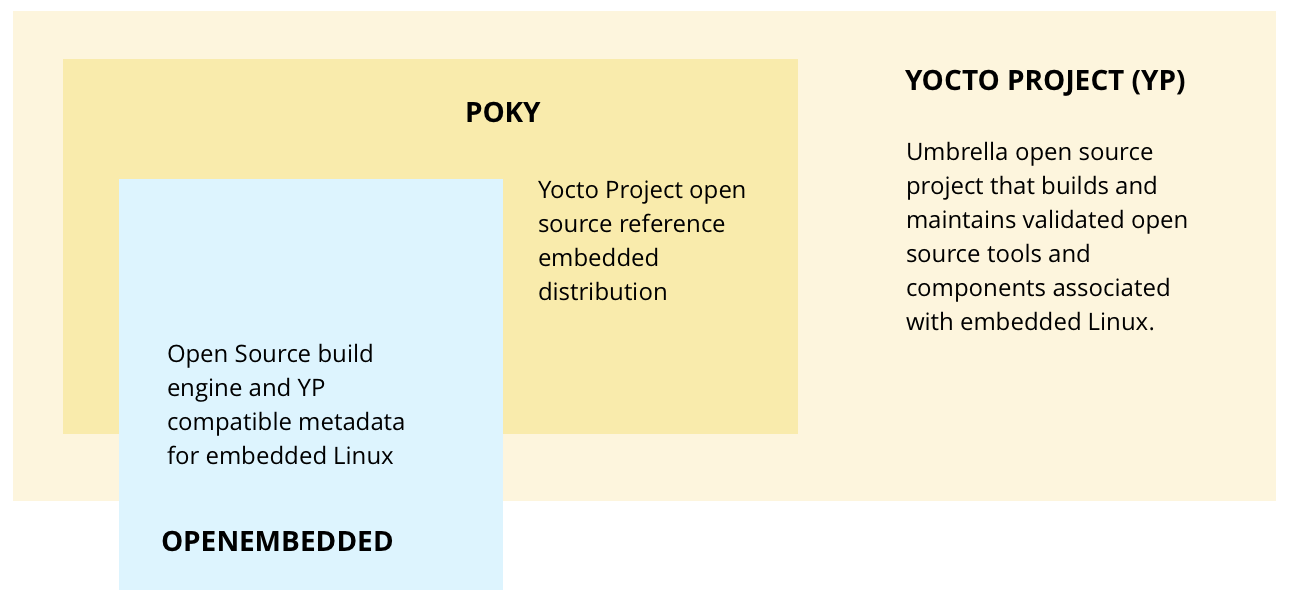
\includegraphics[width=0.60\linewidth]{figs/yocto-overview}
	\caption[Yocto Overview]{Esquema de relación entre Yocto, Poky y OpenEmbedded.}
	\label{fig:yocto_overview}
\end{figure}

\paragraph{}Al principio, Yocto puede resultar ser conceptualmente difícil de entender
ya que su campo de aplicación puede ser muy variado. En este sentido, puede usarse tanto para
la creación de imágenes completas de sistema, creación de \emph{\glsplural{bootloader}}, generación
de sistemas de ficheros (\emph{rootfs}), desarrollo de aplicativos, desarrollo de paquetes
de los aplicativos, desarrollo y/o hacking del kernel y generación de  \emph{toolchains},
\glslink{SDK}{SDKs} o \glslink{ADT}{ADTs}.

\paragraph{\label{layers} \label{recipes}}Los principales conceptos para enterder el
funcionamiento de Yocto, son;
las capas o \emph{layers}, las recetas o \emph{recipes}, las clases y los ficheros de
configuración. Las \emph{recipes} son un conjunto de instrucciones y configuraciones
usadas para la construcción de un paquete. Por ejemplo, una recipe describe la fuente
del código, los parámetros, el compilador y los parches a aplicar así como la instalación
del paquete en la imagen. Las \emph{layers} son conjuntos de recipes agrupadas por
funciones lógicas que interactúan de manera independiente o con una dependencia bien
documentada. Los ficheros de configuración suelen definir un conjunto de variables
dependientes del entorno que queramos construir. Por último, las clases son partes de
código común entre recetas pensadas para ser reutilizadas.

\paragraph{}En cuanto a las opciones de testing, Yocto dispone de test en tiempo
de compilación así como la posibilidad de arrancar las imágenes generadas en una máquina
virtual QEMU \ref{sec:qemu}.

\subsection{Kas.}\label{sec:kas}

\paragraph{}Kas es una herramienta pensada para configurar proyectos basados en bitbake
de una manera sencilla. Kas proveé un \emph{wrapper} de bitbake con comandos de más alto
nivel. Resuelve las tareas de resolución de dependencias, de configuración y de
generación que usualmente suelen hacerse a mano y dejarse documentadas. Yocto
\ref{sec:yocto} utiliza bitbake como motor de generación, por tanto, Kas puede ser
utilizado en proyectos basados en Yocto.
\cite{kas}

\section{QEMU.}\label{sec:qemu}

\paragraph{}Qemu es un emulador de hardware de código abierto capaz de interoperar con
\gls{KVM} para arrancar máquinas virtuales con un rendimiento casi nativo.
\cite{qemu}

\paragraph{}Qemu dispone de los siguientes modos de funcionamiento:

\begin{itemize}
	\item User-mode emulation.
	\item System emulation.
	\item \gls{KVM} Hosting.
	\item Xen Hosting.
\end{itemize}

\begin{figure}[h]
	\centering
	
\includegraphics[width=0.50\linewidth]{imgs/qemu-logo}
	\caption[Qemu Logo]{Logo de QEMU.}
	\label{fig:qemu}
\end{figure}

\paragraph{} El modo ``User-mode emulation'' permite que una sola aplicación compilada
para una arquitectura diferente a la del resto del sistema arranque mediante la ``traducción''
de instrucciones en tiempo real.

\paragraph{} El modo ``System emulation'' es el más común. Se utiliza para simular una
computadora completa, incluidos sus periféricos. Qemu tiene la capacidad de albergar
sistemas operativos Linux, Solaris, Microsoft Windows, DOS y BSD.

\paragraph{} Los modos ``\gls{KVM}'' y ``\gls{XEN}'' son variaciones del modo ``System
emulation'' en el que se simula más o menos hardware con cada uno de los hipervisores cuyo
nombre coincide con el nombre del modo.

\section{Docker.}\label{sec:docker}

\paragraph{}Docker es una herramienta de gestión de contenedores. Dichos contenedores son
una capa de aislamiento a nivel de aplicación que utilizan los recursos del Kernel de Linux
tales como espacios de nombres. A pesar de que no supone un aislamiento tan fuerte como
el que proporcionan las máquinas virtuales, la principal ventaja de los contenedores es
que son mucho más livianos en cuanto a la necesidad de recursos de memoria, disco y computación.
\cite{docker}

\paragraph{} Docker permite empaquetar aplicaciones y todas sus dependencias, de esta
forma tienen una gran capacidad de portabilidad y flexibilidad con respecto al sistema
operativo dónde se ejecuten.

\begin{figure}[H]
	\centering
	
\includegraphics[width=0.50\linewidth]{imgs/docker-logo}
	\caption[Docker Logo]{Logo de Docker.}
	\label{fig:docker}
\end{figure}

\paragraph{} En nuestro caso, Docker nos va a ayudar a empaquetar todo el entorno de
desarrollo y sus dependencias para que su puesta en marcha sea inmediata, también buscará
evitar la heterogeneidad entre los entornos de desarrollo de los diferentes desarrolladores,
así como tener un control de versiones de las propias dependencias y de las variables
de entorno del sistema.

\section{Flutter.}\label{sec:flutter}

\paragraph{} Flutter es un entorno de desarrollo o \gls{SDK} de aplicaciones. El principal
objetivo de Flutter es facilitar la creación de interfaces de usuario que se adapten a
cualquier pantalla y a cualquier dispositivo. En ese sentido, permite que con un sólo
código fuente común se puedan generar aplicaciones para muchos entornos: Android, iOS,
Linux, Windows, Fucsia, etc.
\cite{flutter}

\paragraph{} Flutter sigue la filosofía de programación basada en objetos, y como está pensado
fundamentalmente para entornos gráficos, todos los objetos en Flutter son \gls{Widgets}.

\begin{figure}[h]
	\centering
	
\includegraphics[width=0.50\linewidth]{imgs/flutter-logo}
	\caption[Flutter Logo]{Logo de Flutter.}
	\label{fig:flutter}
\end{figure}

\paragraph{} Gracias a su capacidad para hacer la \gls{cross-compile} sencilla, resulta
ser increiblemente práctico para su uso en aplicaciones embebidas. Permite el desarrollo
de forma aislada del hardware así como el testing de la aplicación. En el apartado
gráfico destaca la persistencia visual entre la interfaz en entornos de desarrollo y
entornos embebidos.

\paragraph{} Está escrito en el lenguaje de programación Dart \ref{sec:dart} y ha sido
desarrollado por Google.

\subsection{Dart.}\label{sec:dart}

\paragraph{}Dart es un lenguaje de programación orientado a objetos de alto nivel.
Está optimizado para interfaces de usuario y para aumentar la productividad de desarrollo,
ya que permite el ``hot debugging''. Una técnica que posibilita cambiar sólo los objetos cuyo
codigo ha sido actualizado, manteniendo el resto en mitad de una sesión de depuración.
\cite{dart}

\paragraph{}Dart permite compilarse en código máquina para tener un rendimiento similar al
de aplicaciones nativas o traducirse a otros lenguajes considerados nativos en sus campos
como por ejemplo JavaScript para su uso en entornos web. Todo eso lo convierte en un
lenguaje de programación multiparadigma que permite el desarrollo tanto del \gls{front-end}
como del \gls{back-end}.

\begin{figure}[H]
	\centering
	
\includegraphics[width=0.50\linewidth]{imgs/dart-logo}
	\caption[Dart Logo]{Logo de Dart.}
	\label{fig:dart}
\end{figure}

\section{Qt.}\label{sec:Qt}

\paragraph{}Qt es un \gls{framework} the interfaces de usuario muy popular y extendido,
se utiliza, fundamentalmente, en sistemas embebidos de cualquier ámbito, desde impresoras
hasta sistemas de armamento. Esto es así porque dispone de \glsplural{API} en C++ y en
Python y ofrece una gran calidad de recursos gráficos y de herramientas. Por ejemplo,
su \gls{IDE} qtCreator facilita muchísimo el desarrollo, ofrece licencias gratuitas para
programas de código abierto, y está muy bien documentada.

\paragraph{}Hasta hace unos años ha sido el framework rey de los sistemas embebidos, pero
con la reciente llegada de \hyperref[sec:flutter]{Flutter} \ref{sec:flutter} a entornos
de escritorio y distribuciones embebidas, puede suponer un cambio de tendencia.

\begin{figure}[H]
	\centering
	
\includegraphics[width=0.30\linewidth]{imgs/qt}
	\caption[Qt Logo]{Logo de Qt}
	\label{fig:qt}
\end{figure}


\section{React Native.}\label{sec:react}

\paragraph{}React Native es una librería basada en la librería React que a diferencia
de ésta, la compilación genera una aplicación nativa para sistemas iOS o Android. Al
estar desarrollada en JavaScript se está convirtiendo en una de las librerías gráficas
más populares. Además permite crear web apps que pueden correr como servicios en local
y ser visualizadas con la ayuda de un navegador web. Existen adaptaciones mediante las
librerías de \hyperref[sec:Qt]{Qt} \ref{sec:Qt} que pueden llevar estás aplicaciones
gráficas a sistemas Linux. Desde un punto de vista práctico, solo sería recomendable
esta opción para \gls{ports}, ya que al no tener un rendimiento nativo y necesitar
adaptadres estamos malgastando los recursos, los cuales suelen ser escasos en los sistemas
embebidos.

\begin{figure}[H]
	\centering
	
\includegraphics[width=0.30\linewidth]{imgs/react-logo}
	\caption[React Logo]{Logo de React}
	\label{fig:react}
\end{figure}

\section{Vagrant.}\label{sec:vagrant}

\paragraph{}Vagrant es un gestor de máquinas virtuales propiedad de HashiCorp que automatiza
su creación y proporciona una interfaz de alto nivel para su gestión, funciona con máquinas
virtuales de VMWare, VirtualBox, AWS, etc. El propósito fundamental de Vagrant es el de
replicar los entornos de ejecución y de desarrollo de forma automática, y que las pruebas
y el desarrollo sean lo más fieles a los entornos de producción de una manera sencilla.

\paragraph{}Su uso resulta muy similar al de \hyperref[sec:docker]{Docker} \ref{sec:docker}
sólo que en este caso se administran máquinas virtuales en vez de containers. Posiblemente
la popularidad de docker ha hecho que Vagrant haya quedado en segundo plano. Otra razón,
por la que Vagrant no ha terminado de ser muy popular es la dependencia con tecnologías
externas de máquinas virtuales, muchas de ellas con necesidad de licencias comerciales,
así como el uso de hipervisores.

\begin{figure}[H]
	\centering
	
\includegraphics[width=0.50\linewidth]{imgs/vagrant-logo}
	\caption[Vagrant Logo]{Logo de Vagrant}
	\label{fig:vagrant}
\end{figure}

\section{Ansible.}\label{sec:ansible}

\paragraph{}Aunque Ansible es confundido muchas veces con \hyperref[sec:docker]{Docker} \ref{sec:docker}
o con \hyperref[sec:vagrant]{Vagrant} \ref{sec:vagrant} aunque resulta ser una tecnología
totalmente diferente. Ansible es una plataforma de software libre para la administración
de equipos. Permite la administración multi-nodo de forma remota y por lotes. Mediante
un equipo orquestador, se puede automatizar el resto de nodos. Se basa en colecciones
de libros de jugadas o \emph{playbooks}.

\paragraph{}Una de las características principales de Ansible es que no tiene ninguna
dependencia salvo la de Python, la cual es asumible ya que la mayoría
de distribuciones Linux trae Python por defecto.

\paragraph{}En nuestro caso, el entorno de desarrollo traerá los playbooks necesarios
para la instalación de las dependencias. Están escritos en playbooks en vez de en scritps
corrientes para poder integrarse en sistemas remotos de administración fácilmente. Desde
el punto de vista de operaciones, Ansible resulta muy conveniente para pasar la configuración
de los entornos de desarrollo como \gls{IaaC} y por tanto usar control de versiones para
la adminsitración y configuración de equipos. En un entorno empresarial real, estos
playbooks posiblemente estarían en un repositorio distinto y se ejecutarían con permisos
de administrador automáticamente, evitando que el usuario necesite el acceso de superusuario.

\paragraph{}Podríamos comparar Ansible con herramientas de Microsoft de gestión remota,
aunque ésto no supone una barrera para que ansible se integre con herramientas de Microsoft
como \emph{Active Directory}.

\begin{figure}[H]
	\centering
	
\includegraphics[width=0.30\linewidth]{imgs/ansible-logo}
	\caption[Ansible Logo]{Logo de Ansible}
	\label{fig:ansible}
\end{figure}

\section{Visual Studio Code.}\label{sec:vscode}

\paragraph{}Visual Studio Code o VSCode abreviadamente es un \glslink{IDE}{IDE} multiplataforma
de código abierto desarrollado por Microsoft. Es un \glslink{IDE}{IDE} ligero y modular
que permite el desarrollo de software en casi todos los lenguajes de programación mediante
la instalación de \gls{plugins}.

\paragraph{}VSCode se puede personalizar completamente al uso requerido en cada caso,
mediante archivos que añaden funcionalidad al \glslink{IDE}{IDE} en tiempo de ejecución
y dependiendo del proyecto abierto. Por ejemplo, un repositorio de Yocto, podría tener unos
ficheros que definieran las tareas más comunes para la generación de Yocto.

\begin{figure}[H]
	\centering
	
\includegraphics[width=0.30\linewidth]{imgs/vscode-logo}
	\caption[Visual Studio Code]{Logo de Visual Studio Code.}
	\label{fig:vscode-log}
\end{figure}

\paragraph{}En muchas ocasiones Visual Studio Code resulta un programa muy conveniente
para su uso como editor básico de texto, al poder tener disponibles todas las características
avanzadas de edición, propias de los programas de edición de código. En el que además,
tenemos una disposición de ventanas manejable con una o más terminales disponibles.

\paragraph{}Por ejemplo, para el desarrollo de Yocto puede ser utilizado cualquier editor
de texto, desde gedit hasta vim en conjunto con cualquier programa de terminal para lanzar los
comandos y probar nuestros cambios. Sin embargo, tener ambas cosas organizadas en la misma
vista, pudiendo tener un árbol de ficheros y varios ficheros abiertos organizados en pestañas
hace que el desarrollo sea más cómodo.


\begin{figure}[H]
	\centering
	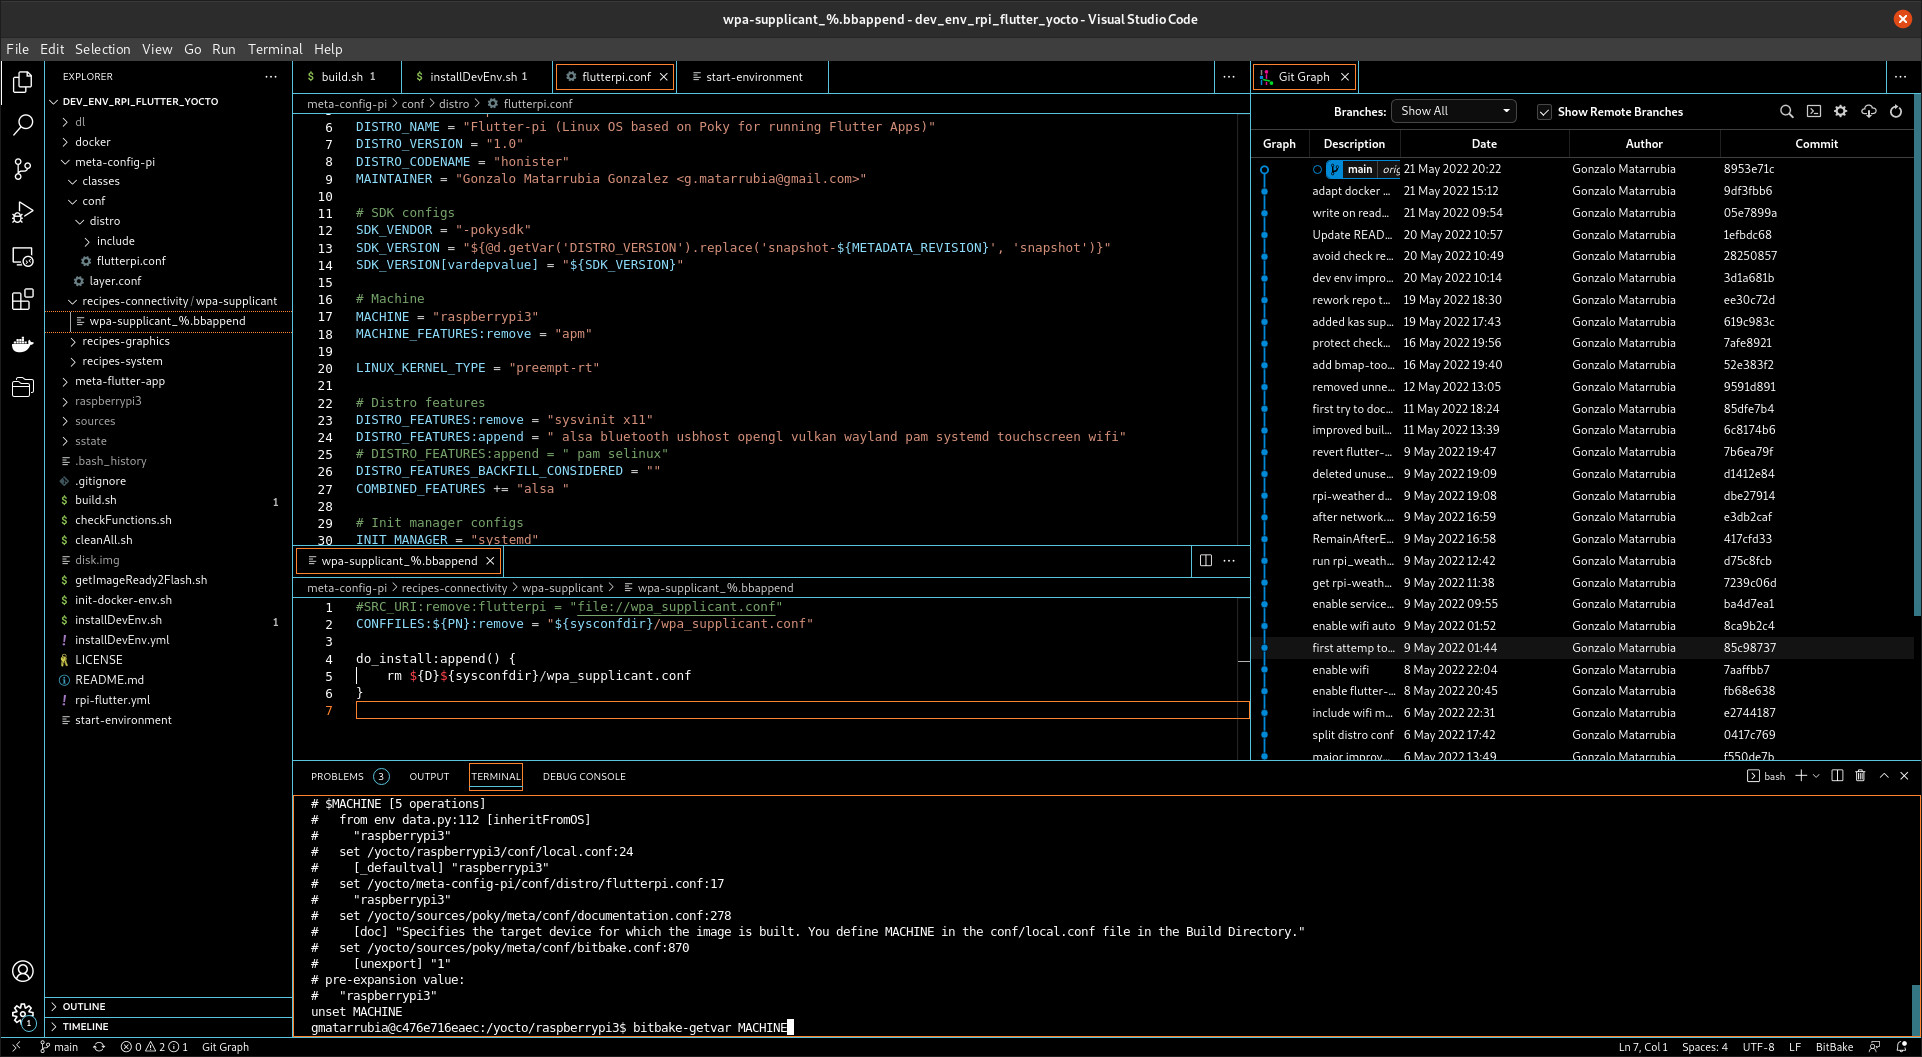
\includegraphics[width=0.90\linewidth]{imgs/vscode-perspective}
	\caption[VSCode yocto]{VSCode usado con Yocto.}
	\label{fig:vscode-perpective}
\end{figure}

\paragraph{}Por su soporte, por su integración con Flutter y todas las razones descritas
anteriormente, hacen de Visual Studio Code el editor perfecto para los entornos de desarrollo
de Flutter y Yocto.

%las referencias a artículos se ponen con \cite,
%las referencias a glosario \gls,
%y las referencias a ecuaciones \eqref
%las referencias a imgenes, tablas o figuras o secciones
% se ponen con \ref (sólo número) o con \hyperref[sec:X]{text}